% Chapter Template

\chapter{Methods} % Main chapter title

\label{Methods} % Change X to a consecutive number; for referencing this chapter elsewhere, use \ref{ChapterX}

%----------------------------------------------------------------------------------------
%	SECTION 1
%----------------------------------------------------------------------------------------

\section{Data collection and preprocessing}


\subsection{Study site}

The audio data used in this study was collected primarily by Jenna Lawson at a study site in the Osa Peninsula, Costa Rica (Figure ~\ref{fig:peninsula_map}). This 2,500 km$^2$ site sits in a particularly diverse region, containing approximately 2.5\% of the world's species on less than 0.001\% of its land area. Three national parks, Corcovado, Piedras Blancas and the Terreba-Sierpe wetlands, and one forest reserve, are represented within this study site. However, protection is not continuous throughout this area as the expanding human population has led to the inevitable landscape alteration brought about by agriculture and urbanisation.

\begin{figure}
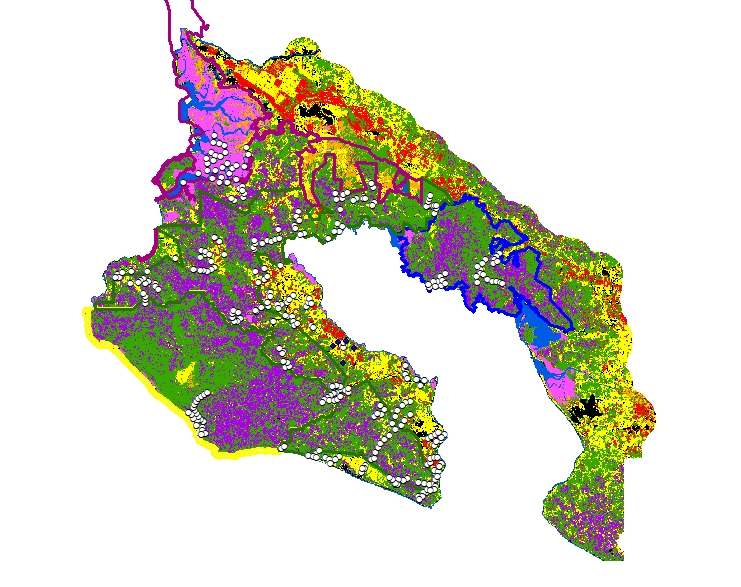
\includegraphics[width=1.2\textwidth,center]{Figures/peninsula_map}\caption[Map of Osa Peninsula]{Map of the study site in the Osa Peninsula \cite{Lawson2019} (NEED KEY/AREAS MARKED)}\label{fig:peninsula_map}
\end{figure}

\subsection{Sampling}

The Costa Rican government have produced a grid system to aid scientific research and conservation efforts in this area, consisting of 240 4x4 km$^2$ zones. This system was extended by Jenna to include the wetland region and 52 zones were removed as we are only interested in the zones that fall within or around the national parks and forest reserve. From the remaining 188 zones, 45 were randomly selected in a stratified manner to ensure good coverage of the region and appropriate representation of the national parks, forest reserve and unprotected land. In all 45 locations, 10 audio recording devices were installed at a minimum distance of 500m from each other to ensure independence of recordings. These 10 locations were also selected using random stratified sampling, ensuring fair representation from each habitat type. Where possible, trails and other areas of high human density were avoided. Each location was assigned to one of ten overall regions within the study site.

\subsection{Recording}

Audio recordings were gathered using AudioMoth devices and were set to record for six consecutive days. Each device was set to record for three periods a day, 0500-0930, 1400-1830 and 2100-0300, chosen to coincide with the peak activity levels of \textit{A. geoffroyi} and their associated poaching. Sound was recorded continuously during these periods at a sample rate of 48 kHz and devices were contained in waterproof casing to avoid damage. Every minute of audio data was saved in a separate file with the filename being a Unix hexadecimal timestamp.


\subsection{Subsetting}

Of the ten regions captured in this dataset, six were selected for this analysis to ensure adequate processing time was available. The selected regions are known to be particular hotspots for illegal activity. Similarly, to minimise computational and manual expense, two sensors were selected at random from these six regions to be used for this analysis. This subset still includes 960 hours of audio data and represents 60\% of the available regions and 40\% of the available audio sensors within those regions.

\subsection{Training data}

\cite{Hill2018} provided the labelled audio data used in their study which was used in this study to train the CNN. The data was collected using 36 AudioMoth devices in the tropical rainforests in Pook's Hill Reserve, Belize. The devices covered 13 sites and were placed 200 m apart from each other. Controlled gunshots were set off by the research team and were labelled as positives in the dataset through visual inspection of spectograms. The detection algorithms used were able to detect 66\% of gunshots up to 500 m away and 50\% up to 1 km away. Devices facing towards the gunshot were 80\% more likely to detect it than those facing away.



\section{Machine learning}

All coding was carried out using either Python (3.6.8) or bash (4.4.20), on an Ubuntu (18.04.3) operating system. For the training data, each audio file was split into four second clips using the pydub (0.23.1) Python module. Each clip was then plotted as a 60x60 mel-spectrogram using the librosa (0.7.0) Python module.\\

\noindent The CNN was then trained using the Keras (2.2.4) Python module. Mel-spectrogram images were imported and the pixel values were normalised to take values between 0 and 1 (rather than 0 and 255) as this has been shown to improve convergence and stability \citep{Liao2016}. The data was split randomly into training and validation data in the ratio 3:1 as this has been shown to be appropriate for a dataset of this size \citep{Guyon1997}. The seed for random number generation was set to ensure repeatability.

\subsection{Convolutional Neural Network}

The CNN was constructed using \cite{Chollet2016}'s tutorial as a template. The first layer was a convolutional 2D kernel which is convolved with the input layer to produce a tensor of outputs, the input layer being $n$ spectrograms of 64x64x3 size. It contained 32 nodes which determines the dimensionality of the output space and a 3x3 convolutional window. A 'relu' activation function was then applied as this was shown by \cite{Glorot2011} to enable better training of deep neural networks, compared to other common activation functions such as the logistic sigmoid. The identified features are then passed through a max pooling layer which determines the most activated presence of each feature within a 2x2 cluster of features. Put simply, this filters out the less important features and keeps the most important ones to be passed to the next layer. In this model, these three layers were repeated in the same order, two further times, with the model then totalling nine layers. The features were then passed to a 'flattening' layer. This is a layer that takes a two-dimensional matrix of features and transforms them into a vector of features than can fed to a neural network classifier, in this case a 'dense' layer composed of 64 fully-connected neurons. These neurons linearly take all the inputs from the previous layer, apply a weight to them and output to the next layer which in this CNN was another 'relu' activation layer. The activation layer output is then passed through a 'dropout' layer, in this case that involved randomly discarding 50\% of nodes in an effort to minimise overfitting. The remaining nodes are put through another 'dense' layer, this time with 2 nodes as this CNN was only being trained in a binary 'gunshot' or 'no gunshot' manner. The output of this 'dense' layer was passed through a final 'softmax' activation layer which is similar to logistic regression but usually used in multi-classification problems. However, it has been shown to be more effective than logistic regression even in binomial classification (FIGURE NEEDED).

\subsection{Training the model}
Initially, the model was trained on the data provided by \cite{Hill2018} by randomly splitting the data into training and test data in a ratio of 70:30. The training and test data was comprised of equal numbers of positive (gunshots) and negative (no gunshot) spectra as imbalanced ratios have been previously shown to be ineffective \citep{Kim2018} and preliminary experimentation on this dataset confirmed this. This model was then fed the subset of data from the Osa Peninsula and the returned 'gunshots' were manually checked for authenticity. The validated gunshots were used to retrain the model in the same manner, before being fed data from the Osa Peninsula that had not already been used to train the model. The model was retrained a further two times, once with a combined training dataset of both \cite{Hill2018} and Osa Peninsula, and another with the Osa Peninsula data, this time the negatives used were the false positives identified originally.
